\chapter{Conclusions and Future Work}
\section{Conclusions}
% TODO: Update conclusions
\noindent As presented in Chapter \ref{chap:stateoftheart} Section \ref{section:MECarch} several architectures have been proposed in the \acrshort{MEC} context that present complex optimization problems of managing how to distribute tasks between \acrshort{UE}s and \acrshort{MEC} servers. Due to the high dimensional complexity and uncertain networking conditions, classical offline optimization algorithms fail to effectively manage these types of problems. As a solution to this, a review of the state of the art in \acrshort{DRL} and its application to these \acrshort{MEC} challenges was made in Chapter \ref{chap:stateoftheart} Sections \ref{section:RL}, \ref{section:EE} and \ref{section:RW}. Based on the work done by papers \cite{NUE1mec} and \cite{taskclass1} a more complete system that takes into account the possibility of offloading between a network of heterogeneous \acrshort{UE}s to a network of heterogeneous \acrshort{MEC} servers is proposed. To deal with the increased complexity of taking into account computation, battery, delay and communication constraints in an N to N problem several \acrshort{DRL} algorithms will be tested. As far as the candidate knows, this is the first time that this extended optimization problem is addressed.

\clearpage
\section{Future Work}
% TODO: Replace Work Plan with Future Work
\noindent In order to achieve the proposed objectives, a work plan timeline is presented in the following Gantt chart shown in Figure \ref{ganttchart}. For the production of this report, a literature review was made and an initial simulation, baseline algorithms and simple test suite were implemented. The next step is the implementation of the various \acrshort{DRL} algorithms and their respective testing. The idea behind the order of their implementation comes from starting with the less complex but lower quality algorithms and low complexity test suites and then based on the results increase the problem and solution complexities.

\begin{figure}[h]
  \centering
  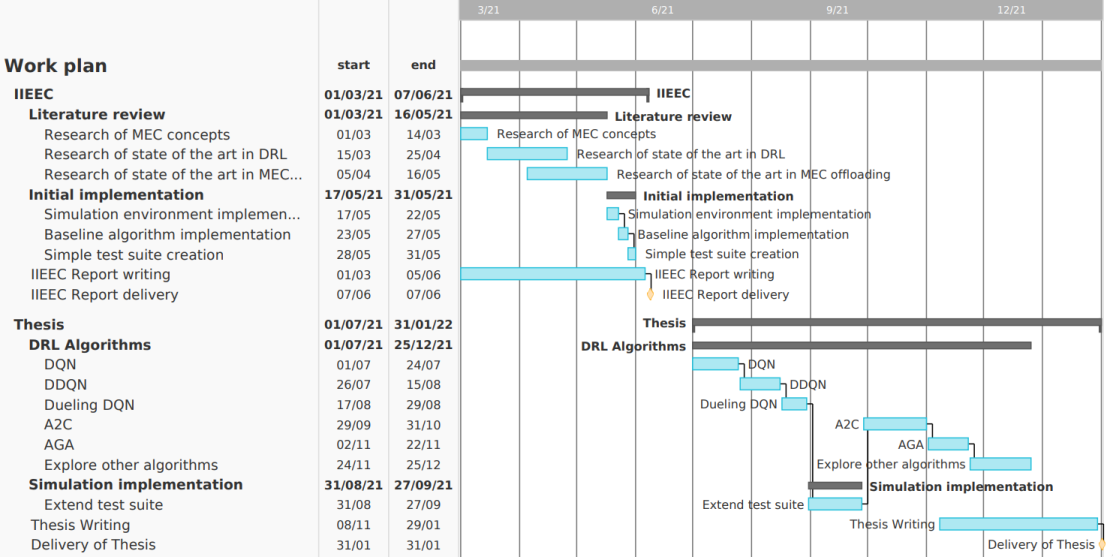
\includegraphics[width=\textwidth]{images/workPlan.png}
  \caption{Gantt chart of work plan} \label{ganttchart}
\end{figure}